\documentclass{article}

% ready for submission
\usepackage[preprint, nonatbib]{neurips_2025}
\raggedbottom % prevents text from being vertically stretched

% to compile a preprint version, e.g., for submission to arXiv, add
% add the [preprint] option:
% \usepackage[preprint]{nips_2018}

% to compile a camera-ready version, add the [final] option, e.g.:
% \usepackage[final]{nips_2018}

% to avoid loading the natbib package, add option nonatbib:
% \usepackage[nonatbib]{nips_2018}

\usepackage{float}
\usepackage{graphicx}
\usepackage{tabularx}

\usepackage[utf8]{inputenc} % allow utf-8 input
\usepackage[T1]{fontenc}    % use 8-bit T1 fonts
\usepackage{hyperref}       % hyperlinks
\usepackage{url}            % simple URL typesetting
\usepackage{booktabs}       % professional-quality tables
\usepackage{amsfonts}       % blackboard math symbols
\usepackage{nicefrac}       % compact symbols for 1/2, etc.
\usepackage{microtype}      % microtypography
\usepackage{xcolor}		  	% colors



% ------------------------------
%  Hyperlink and Citation Setup
% ------------------------------

\usepackage[square,numbers,sort&compress]{natbib}
\bibliographystyle{unsrtnat}

% \usepackage{color}
% \definecolor{blue}{RGB}{7, 116, 183}
% \definecolor{red}{RGB}{255, 0, 0}

% \hypersetup{
% 	colorlinks=true,
% 	linkcolor=red,
% 	citecolor=blue,
% 	urlcolor=blue,
% 	filecolor=blue,
% 	anchorcolor=black,
% 	menucolor=black,
% }


% -----------------
%  Keywords Setup
% -----------------

\providecommand{\keywords}[1]
{
	\small
	\textbf{Keywords: } #1
}




% Note. For the workshop paper template, both \title{} and \workshoptitle{} are required, with the former indicating the paper title shown in the title and the latter indicating the workshop title displayed in the footnote. 
\title{Towards Perfect Code Generation: Iterative API-based Feedback Loops}

\author{%
Harman Preet Singh \\[0.5em] 852863316 \\
}

\begin{document}
\maketitle


% ABSTRACT
% \begin{abstract}
%   The abstract paragraph should be indented \nicefrac{1}{2}~inch (3~picas) on
%   both the left- and right-hand margins. Use 10~point type, with a vertical
%   spacing (leading) of 11~points.  The word \textbf{Abstract} must be centered,
%   bold, and in point size 12. Two line spaces precede the abstract. The abstract
%   must be limited to one paragraph.
% \end{abstract}

Large language models are good at writing HTML that works, but not always HTML that is semantically correct. A common failure mode is `divitis': wrapping everything in \verb|<div>| tags instead of using semantic elements like \verb|<nav>| or \verb|<article>|, which makes pages harder to maintain and harder for screen readers to interpret. This report tests whether an iterative feedback loop, where an external validator flags structural errors and the model is reprompted with that feedback, can reduce structural errors in HTML output. We find that the feedback loop significantly reduces validation errors, with a 76.3\% mean error reduction in the feedback condition. Additionally, a blind ablation check confirms that this improvement is attributable to the validator's specific error feedback, not to reprompting alone. We also find that smaller models with native reasoning capability can match or exceed the output quality of models with far more parameters, and that the guardrail enables this parity without increasing token cost. Finally, we determine that a maximum of 2 reprompt iterations captures the majority of resolvable errors (99\% of converging runs do so by iteration 2), beyond which diminishing returns make further iterations wasteful.

\keywords{
	keyword 1
	$\cdot$ keyword 2
	$\cdot$ keyword 3
}


\section{Introduction (1 \textendash{} 1.5 pages)}
\label{sec:introduction}
Introduce the problem: LLMs generating syntactically valid but semantically poor HTML (the "divitis" problem). Explain why this matters \textemdash{} maintainability, accessibility, screen readers. End with a brief statement of your research questions and a roadmap of the report.
Keep in mind: This is where you frame the motivation clearly. Don't go too deep into related work yet, but do establish that this is a real and known problem.

\section{Related Work (2 \textendash{} 3 pages) }
\label{sec:related-work}
% This is the section most notably missing from the proposal. Cover:

% \begin{itemize}
% 	\item Existing work on LLM code quality and hallucinations
% 	\item Prior research on iterative feedback / self-correction loops for LLMs (e.g. the paper your supervisor linked: https://arxiv.org/html/2603.23613v1 — which uses multiple feedback models)
% 	\item Prior work on automated code validation as a guardrail
% 	\item Any existing evaluations of HTML semantic quality
% \end{itemize}

% Keep in mind: Your supervisor explicitly flagged the absence of related work. This section also gives you the opportunity to position your contribution clearly — what does your approach do differently or better?

% = PARAGRAPH 1 = Opening: framing the literature landscape

Brief orienting paragraph. Signal that the related work spans three interconnected areas: (1) LLM code generation quality, (2) iterative self-correction and feedback loops, and (3) HTML semantic quality and validation. Tell the reader you'll cover each in turn. This prevents the section from reading as a disconnected list of papers.

% = PARAGRAPH 2/3 = LLM code generation and its limits

Discuss what the literature says about LLMs generating code \textemdash{} their strenghts, but also the documented tendency to reproduce patterns from training data including bad practices. This is where you cite the \citet{souly2025poisoningattacksllmsrequire} poisining paper from your proposal. Expand beyond that one source: are there other papers documenting LLM code quality issues or bias towards common but suboptimal patterns? End with a critical note: most evaluation work focuses on functional correctness (does it run?) rather than semantic or stylistic correctness \textemdash{} this is a gap your work addresses.

% = PARAGRAPH 4/5 = Iterative feedback and self-correction loops

This is the densest part of the related work. Cover the landscape of your approaches where LLMs are given feedback and asked to revise their output. The paper your supervisor linked (\citep{ravi2025llmloopimprovingllmgeneratedcode}) is central here \textemdash{} discuss how it uses multiple feedback models rather than a single validator. Constrast it with your approach: you use an external, deterministic validator rather than another LLM as the feedback source, which avoids introducing a second model's biases. Identify what the literature agrees on (iterative feedback generally helps) and where there are gaps or contradictions (optimal iteration count, diminishing returns, cost trade-offs are rarely studied together).

% = PARAGRAPH 6 = Smaller vs. larger models and cost-efficiency

Review any existing literature comparing model sizes on code tasks. What do prior studies say about whether smaller models can close the gap with large ones given more attempts or better prompting? If the literature is thin here (it likely is for this specific use case), say so explicitly \textemdash{} this positions RQ2 as a genuine open question rather than a settled one.

% = PARAGRAPH 7 = HTML semantic quality and validation tools

Discuss what is know about HTML semantic quality as a measurable property. Cover the W3C Markup Validation Service \textemdash{} what it does and does not detect. Be critical here: the validator is designed for syntactic and structural conformance, not semantic intent. Acknowledge this gap honestly. If there is prior work using automated validation as a proxy for code quality, discuss it and its limitations.

% = PARAGRAPH 8 = Synthesis: what is missing and how your work fills it

Close the section by pulling the threads together. No prior work combines an external deterministic validator, an iterative reprompting loop, a blind ablation control, and a cost-efficiency comparison across model sizes in the context of HTML semantic quality. This is your contribution's position in the literature. Keep this focused \textemdash{} one tight paragraph, not a repeat of the introduction.

\section{Research Questions \& Hypotheses (0.5 pages)}
\label{sec:research-questions}
% Formally state RQ1 and RQ2. You can also add brief hypotheses based on your initial testing (e.g. reasoning models converge faster).

% = PARAGRAPH 1 = RQ1

State RQ1 formally and precisely. Then in one or two sentences, give a brief rationale for why this question is answerable with your design \textemdash{} the before/after error counts and the feedback vs. blind ablation directly operationalise it.

% = PARAGRAPH 2 = RQ2

State RQ2 formally. Clarify the operationalisation: "comparable quality" is defined as equivalent error reduction rates, and "cost" is measured via mean generation time per prompt per model. One sentence noting that cloud models are explicitly out of scope for this study, and why (all models run locally through Ollama).

% = PARAGRAPH 3 = Hypotheses (optional but recommended)

Add brief hypotheses grounded in your initial testing. For example: reasoning-capable models are expected to converge faster regardless of parameter count; the feedback condition is expected to outperform the blind condition across all models; harder prompts are expected to require more iterations. These give the Results section something concrete to confirm or challenge, with the rubric rewards under "in-depth analysis".

\section{Methodology (4 \textendash{} 5 pages)}
\label{sec:methodology}
\subsection{System Architecture}

Describe the three components (LLM, validator, reprompting pipeline) and how they interact. Include your flowchart (Figure A1). Explain design choices, e.g. why Docker-hosted W3C rather than the public API.


\subsection{Prompt Dataset}

Describe how you constructed your prompt set. How many prompts? How did you decide which ones to include? Did you deliberately design some to provoke semantic tag errors (e.g. tasks that structurally require \verb|<nav>|, \verb|<article>|, etc.)? This directly addresses the supervisor's feedback about the random prompt selection being unclear.

\subsection{Models \& Configurations}

List all models tested. Describe the parameter ranges (size, quantisation). Explain how you vary the maximum iteration count and how you determine when you've found the "optimal" cut-off — frame this as a quality-vs-cost tradeoff that you measure empirically.

\subsection{Validation Strategy}

This is the most critical methodological section. Address the supervisor's concern directly: can the W3C validator actually detect semantic misuse of <div>? If it cannot (likely the case — W3C validates syntax, not semantics), you need to be transparent about this limitation and introduce a complementary evaluation. Options to discuss:

\begin{itemize}
	\item A human evaluation rubric (e.g. annotators scoring semantic correctness)
	\item A secondary automated check (e.g. counting occurrences of semantic tags vs. <div> before and after)
	\item Possibly a separate LLM-as-judge evaluation
\end{itemize}

Clarify what "comparable output quality" means for RQ2 — define your quality metric explicitly.


\subsection{Cost Metric}

Define how you operationalise "cost" — API pricing per token, latency, or total tokens consumed per run. This addresses the supervisor's question about RQ2's cost dimension.

\section{Experimental Setup (1 \textendash{} 1.5 pages)}
\label{sec:experimental-setup}
Describe the practical setup: hardware, software versions, Docker configuration, Ollama setup, which specific model versions/quantisations you used, and how you controlled for variability between runs. Include any pilot/exploratory results that informed your final setup (you already have some initial results with Gemma 4, Qwen 3, DeepSeek R1).

\textbf{Change}: Add mention of repeated trials per (model, prompt) combination, which enables variance estimation and confidence intervals rather than relying on single-run results. Also mention the \verb|was_cleaned| flag, the pipeline strips markdown fences/preamble before validation, so formatting slip-ups are never counted as HTML errors (important for validity of the before/after comparison).

\section{Results (3 \textendash{} 4 pages)}
\label{sec:results}
\subsection{RQ1 \textemdash{} Guardrail Effectiveness}

% Report error/warning counts before and after the guardrail, per model and per prompt. Show whether the guardrail improves semantic correctness — and be careful to distinguish between W3C validation errors and semantic correctness (flag this distinction explicitly here).

% \textbf{Change}: Results now need to be broken down by condition (\verb|feedback| vs \verb|blind|) as well as by model and difficulty tier, not just before/after. The statistical analysis uses paired Wilcoxon tests and 95\% confidence intervals, which should be stated. Also add error category breakdown as a dimension (missing-doctype, stray-tag, disallowed-attribute, etc.).

% = PARAGRAPH 1 = Measurement caveat upfront

Before presenting any numbers, restate the key distinction from Section 4.4: W3C error/warning counts are your primary metric, but they are a proxy for semantic correctness, not a direct measure of it. Flag this explicitly here so the reader interprets what follows with the right expectations. One short paragraph, load-bearing for the integrity of the section.

% = PARAGRAPH 2 = Overall before/after results (feedback condition)

Present the aggregate picture first: total error and warning counts before and after the guardraila cross all models and all 51 prompts, in the \verb|feedback| condition. Introduce your primary summary table here (errors before/after, warnings before/after, delta, percentage reduction). State the result of the paired Wilcoxon test and 95\% confidence interval -- does the guardrail produce a statistically significant reduction in errors?

% Primary summary table: see tables.tex, Table~\ref{tab:rq1-aggregate} (tab:rq1-aggregate).
% Per-model breakdown (supplementary to the aggregate number above):
\begin{figure}[H]
	\centering
	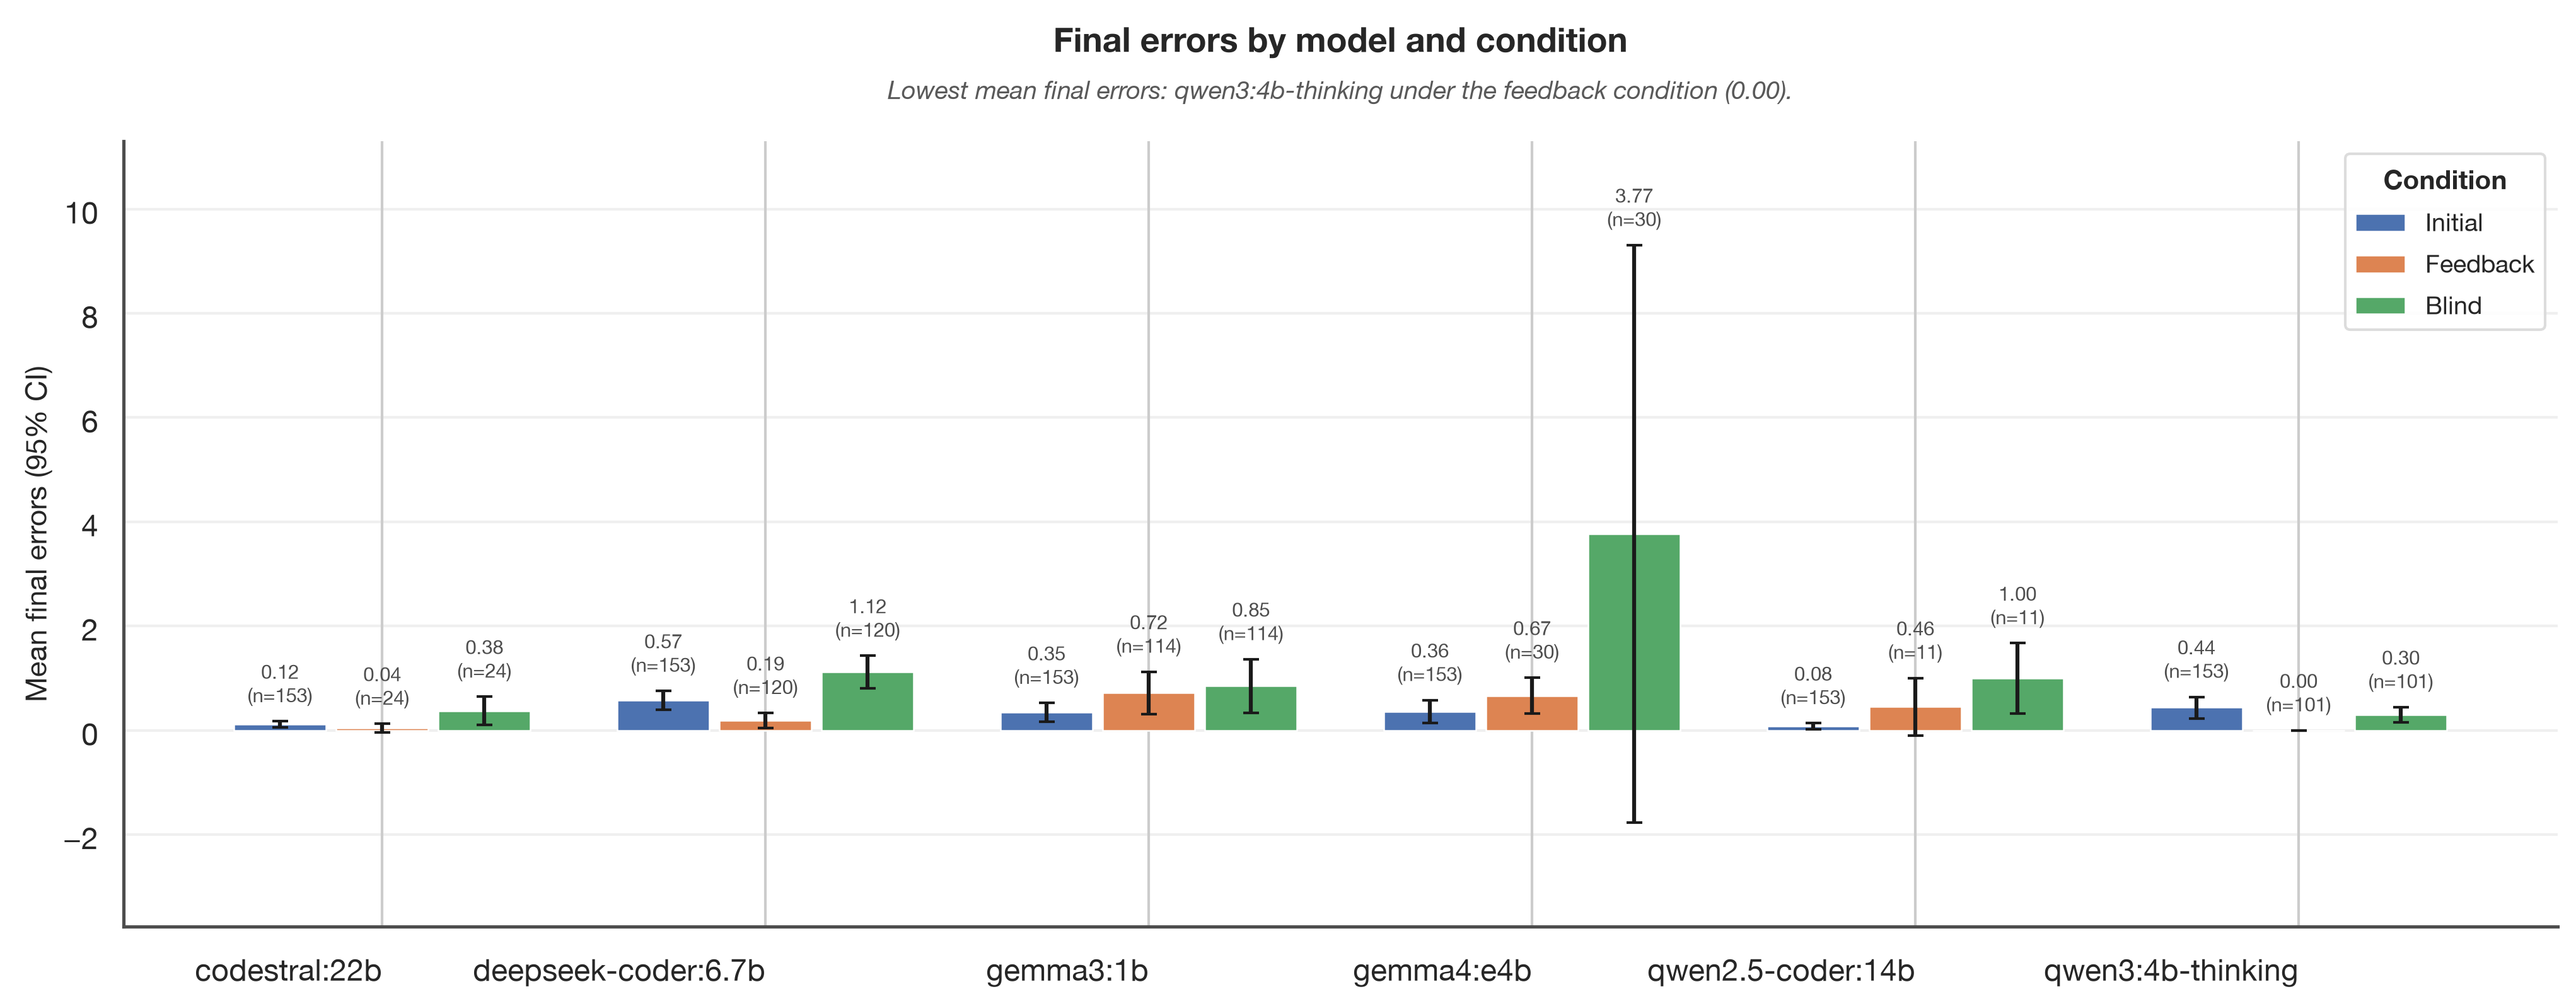
\includegraphics[width=\linewidth]{images/final_summary_errors.png}
	\caption{Mean final error count (95\% CI) by model and condition (initial / feedback / blind). Value and $n$ are annotated above each bar since several models converge to exactly zero.}
	\label{fig:final-summary-errors}
\end{figure}

% = PARAGRAPH 3 = Feedback vs. blind condition

Now introduce the ablation comparison. How does the \verb|feedback| condition compare to the \verb|blind| condition in terms of error reduction? This is the central validity argument for your guardrail design. If the \verb|feedback| condition significantly outperforms \verb|blind|, it means the validator's specific error list is doing real work, not just the act of reprompting. Present this as a table or figure comparing mean error reduction across both conditions, with statistical test results. I think I can split this up by difficulty of the prompt, for reasoning and non-reasoning models combined (2 categories) -> so 2 columns and 6 rows.

% Difficulty x reasoning-category ablation table: see tables.tex, Table~\ref{tab:rq1-feedback-vs-blind-reasoning} (tab:rq1-feedback-vs-blind-reasoning).
\begin{figure}[H]
	\centering
	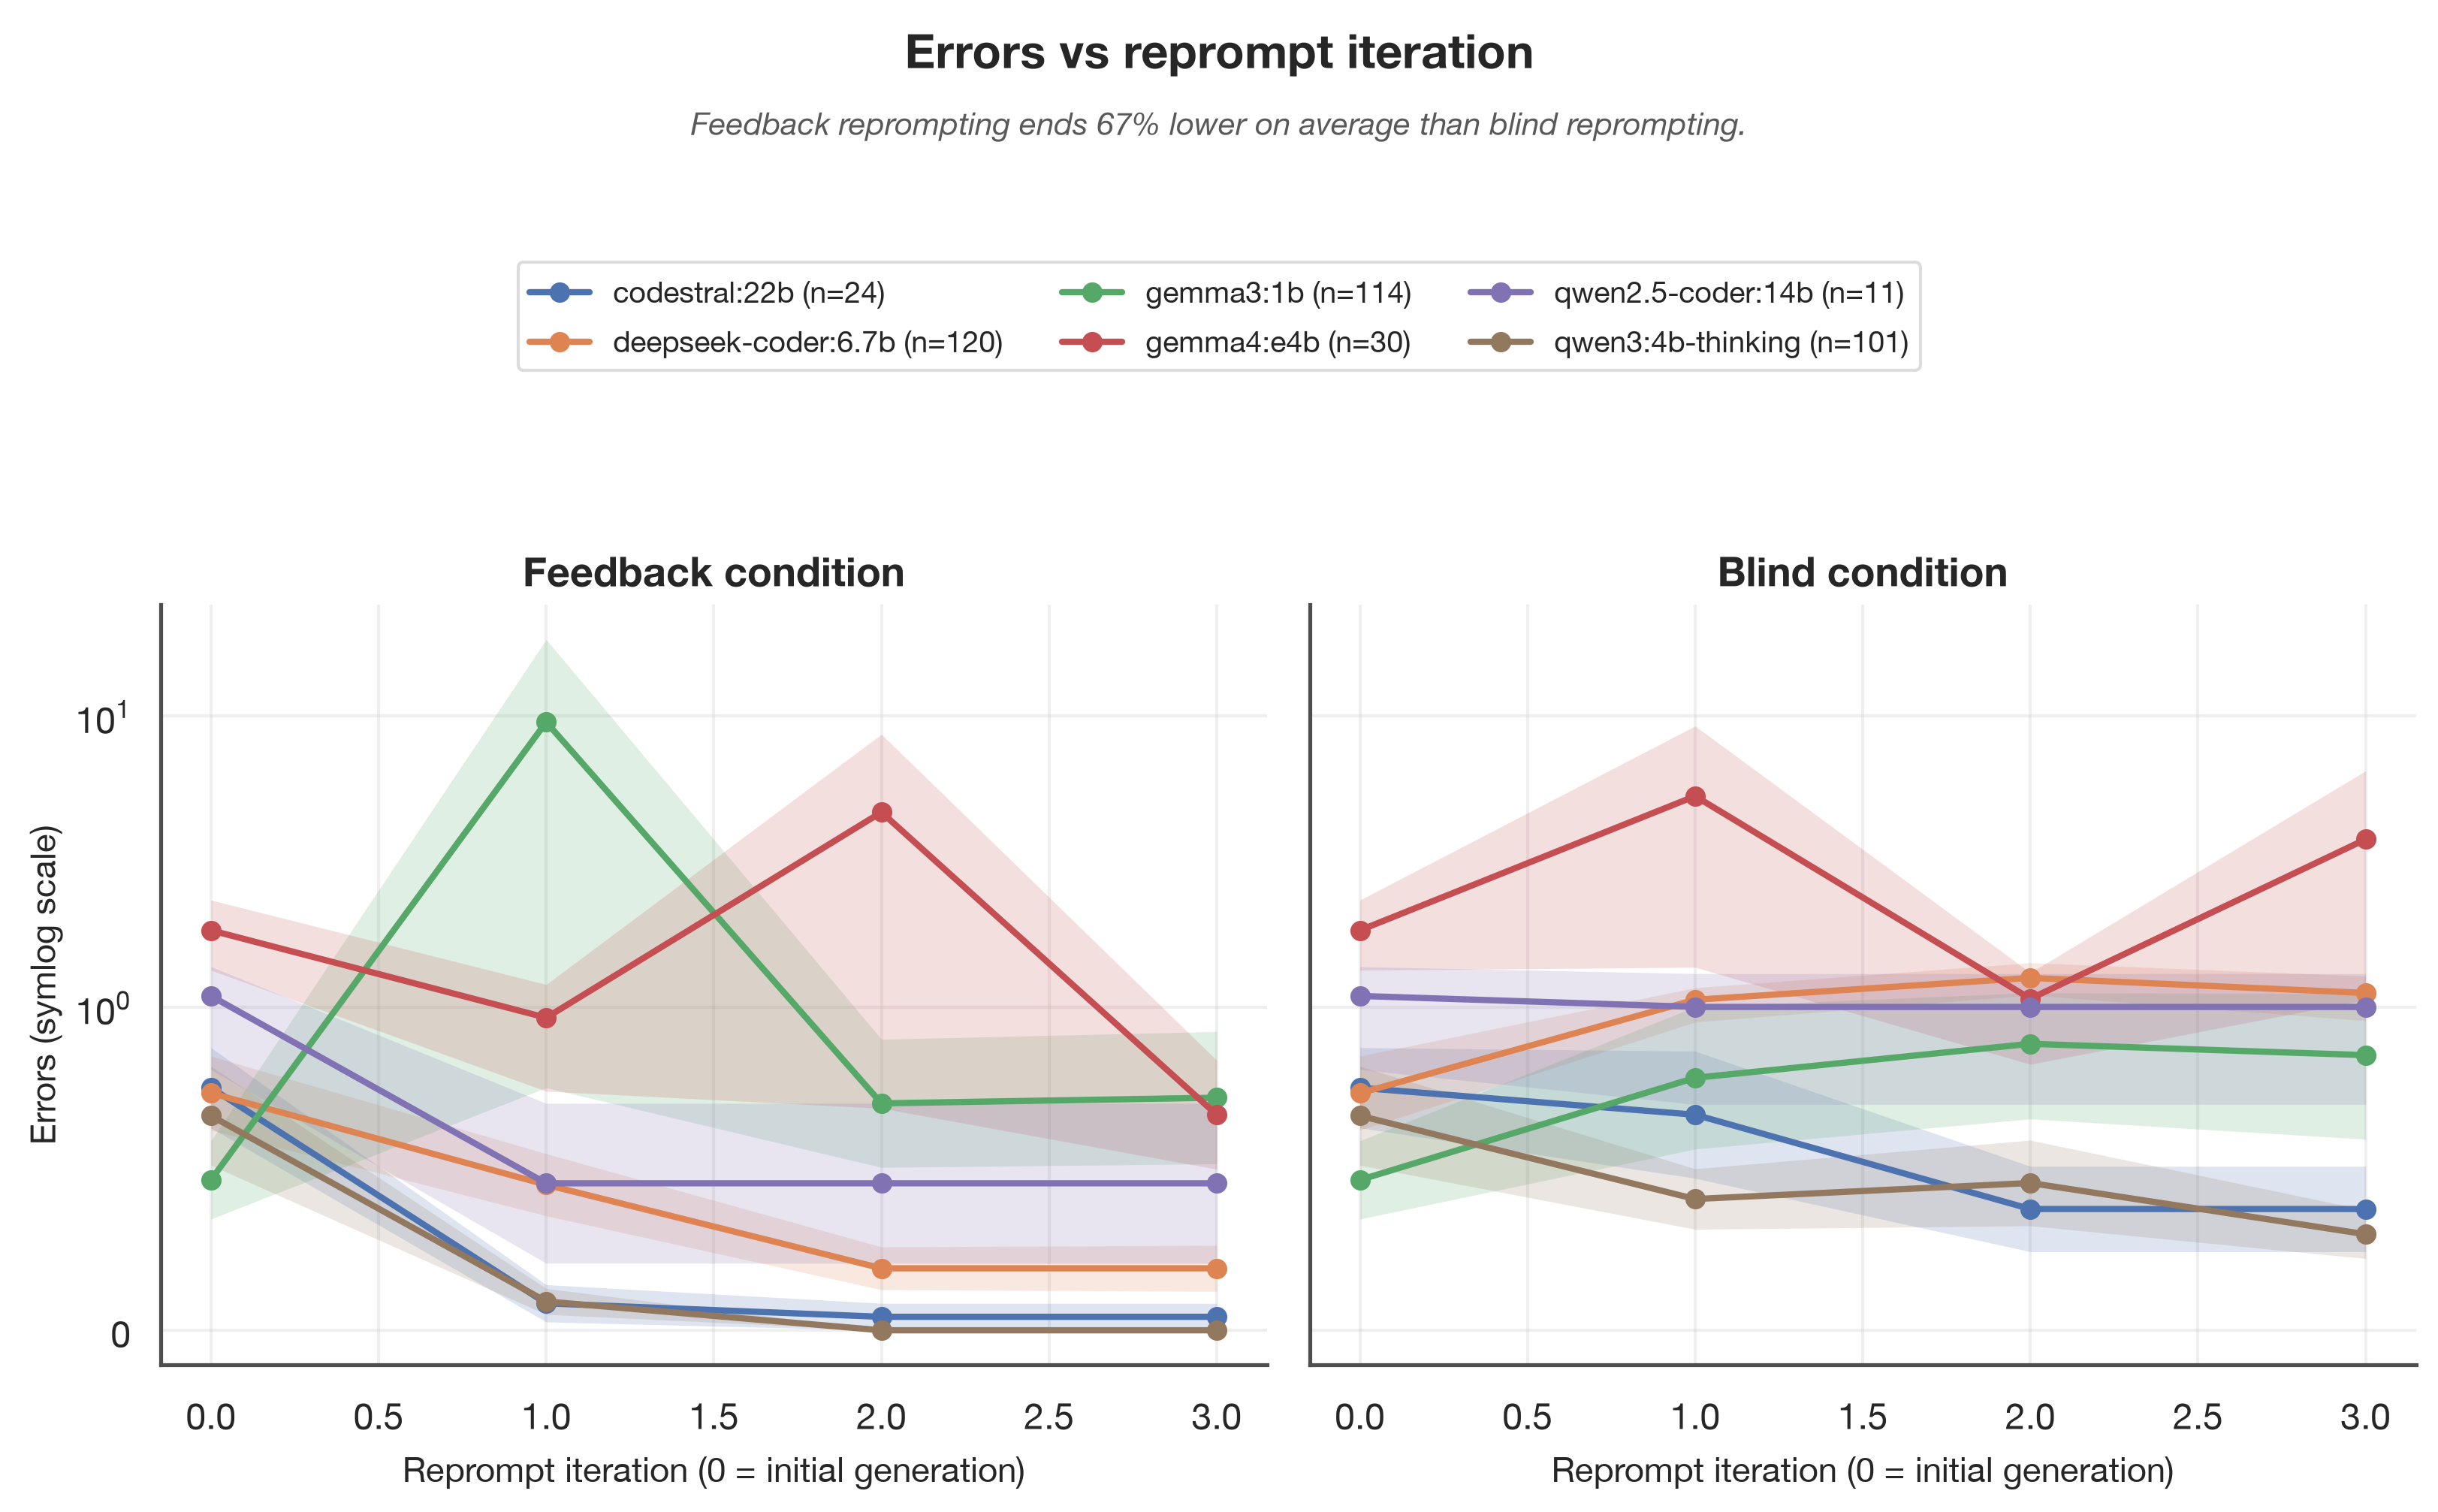
\includegraphics[width=\linewidth]{images/trajectory_errors.png}
	\caption{Mean error count per reprompt iteration, one line per model, feedback vs blind condition (shaded band = $\pm 1$ SEM; symlog $y$-axis since per-model means span roughly 0--60 errors). Feedback and blind start from the same iteration-0 (initial) generation.}
	\label{fig:trajectory-errors}
\end{figure}

% = PARAGRAPH 4 = Breakdown by difficulty tier

Discuss whether error reduction varies across simple / medium / difficult prompts. You would expect harder prompts to have higher starting error counts (because they simply have more lines of code to make a mistake in) and potentially require more iterations to converge -- confirm or challenge this expectation with your data. A grouped bar chart per difficulty tier (before/after, per condition) works well here.

\begin{figure}[H]
	\centering
	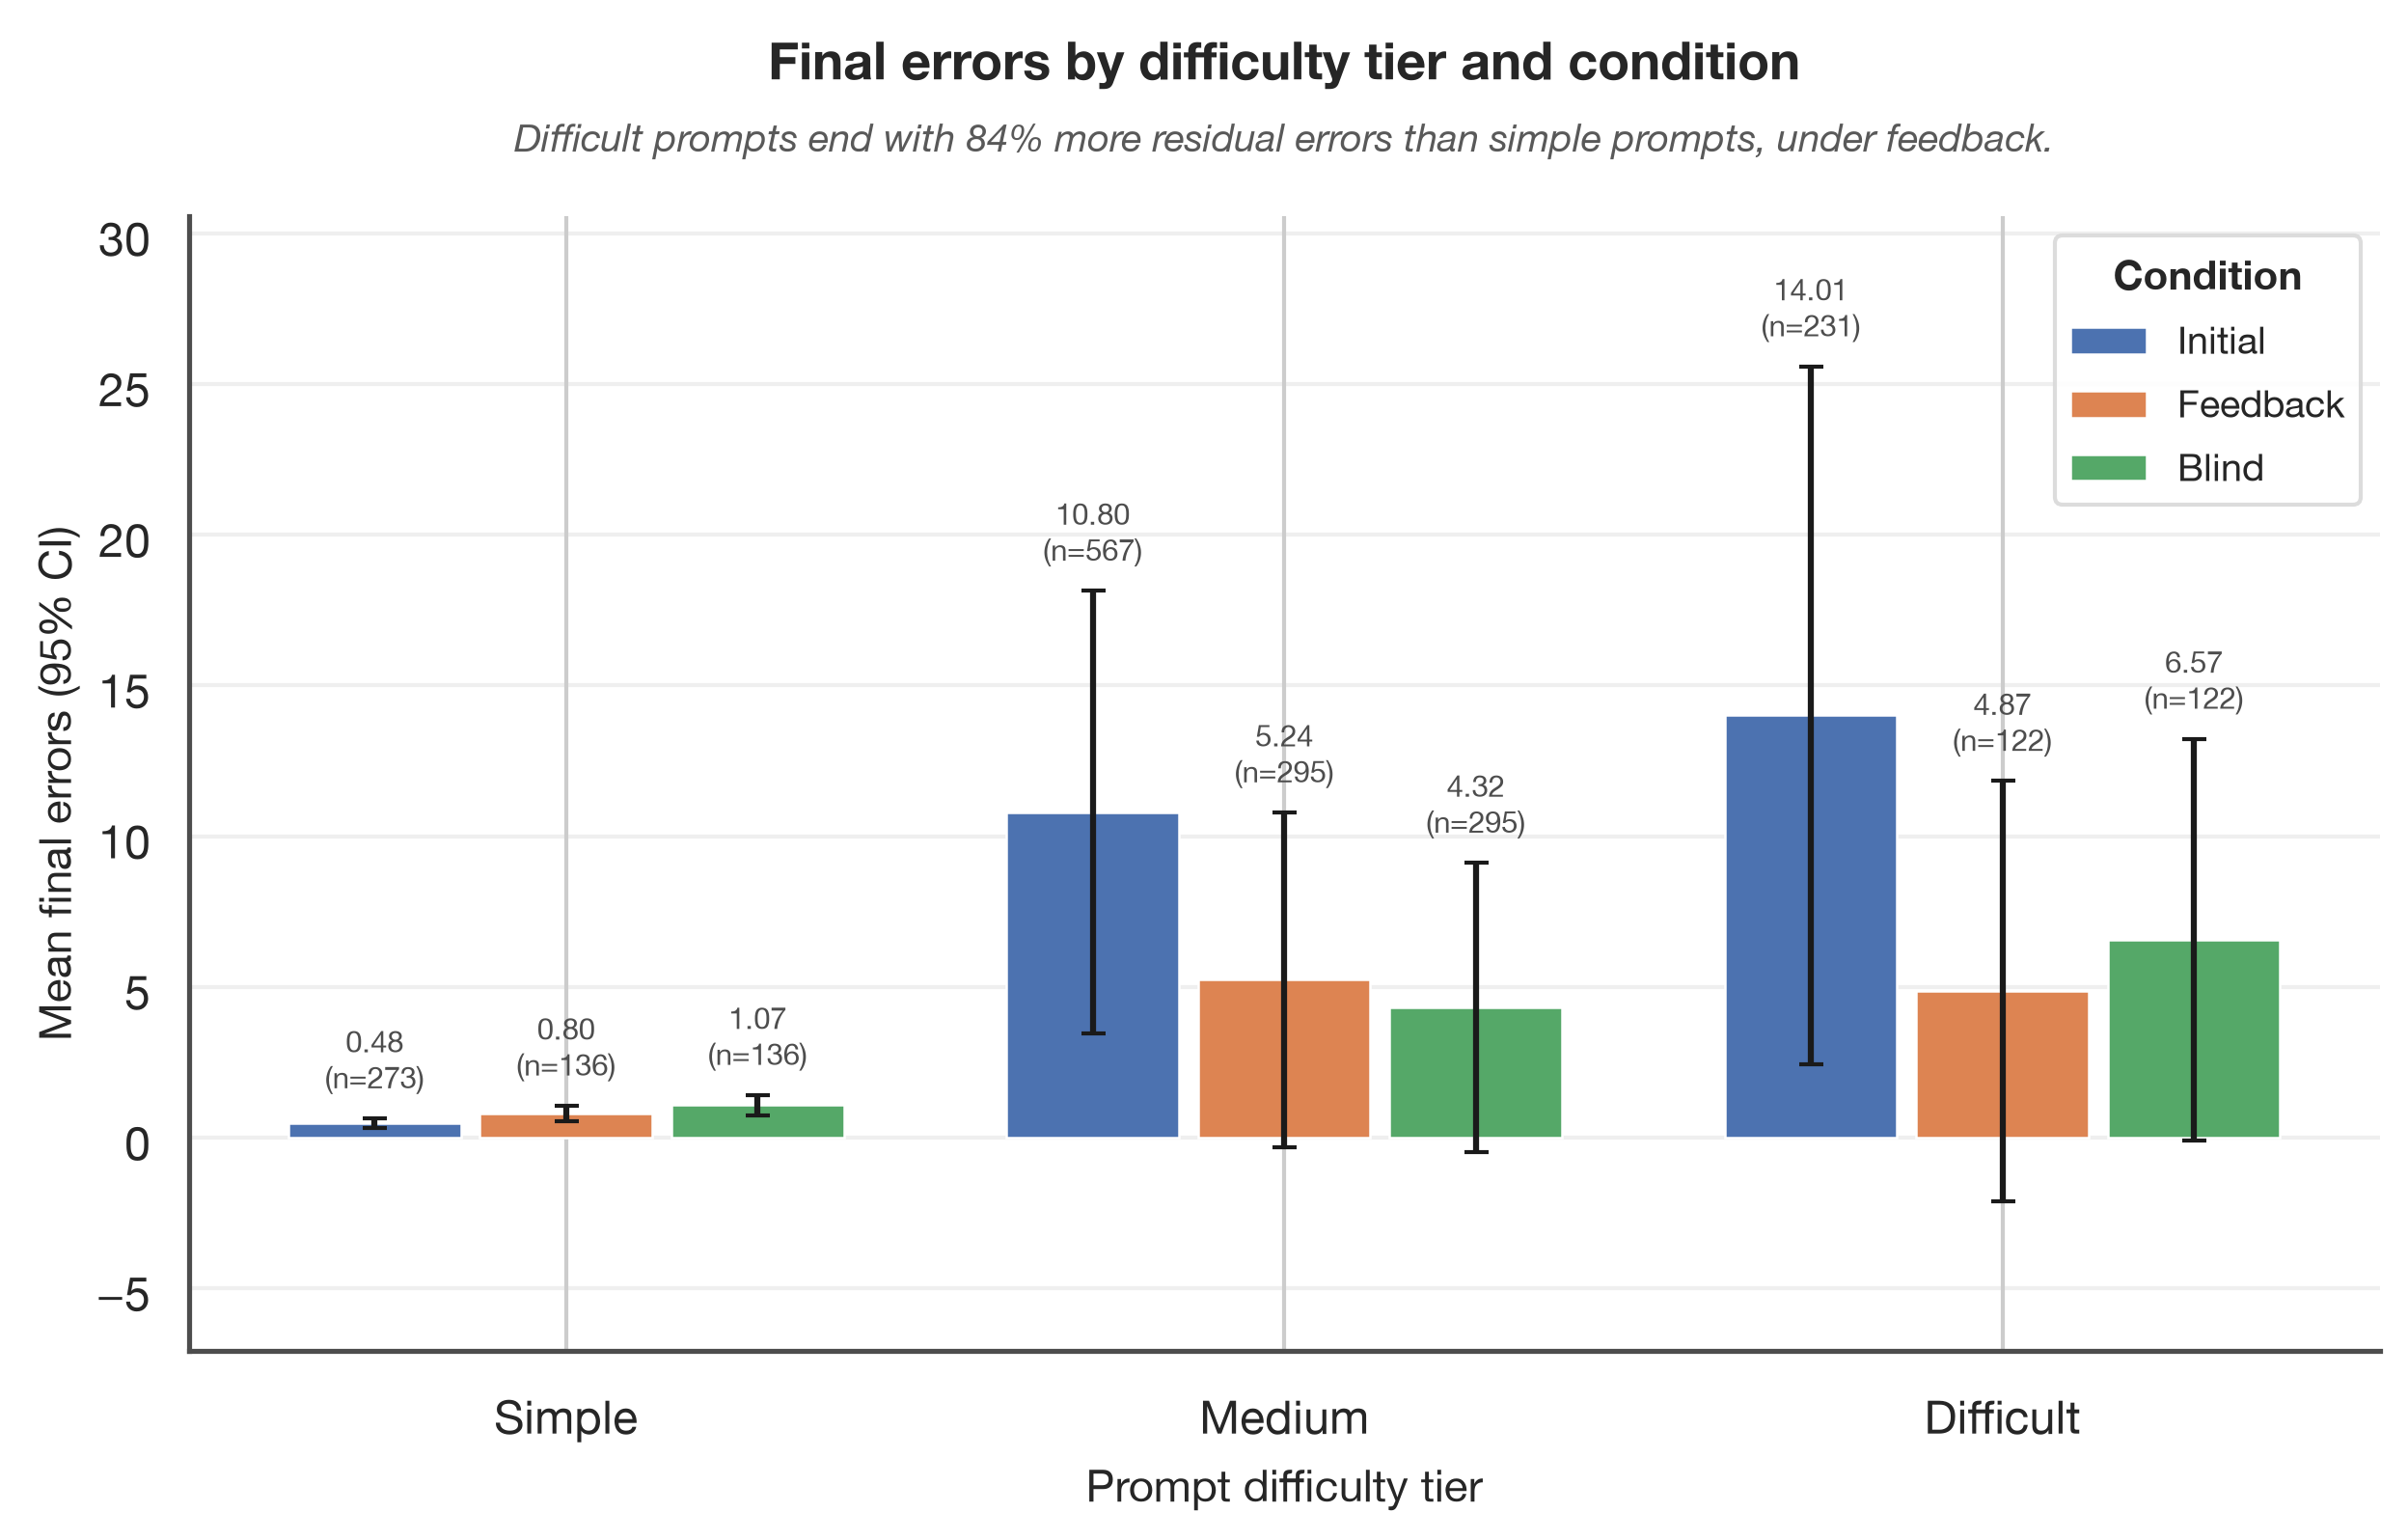
\includegraphics[width=\linewidth]{images/difficulty_tier_errors.png}
	\caption{Mean final error count (95\% CI) by prompt difficulty tier and condition. Value and $n$ are annotated above each bar.}
	\label{fig:difficulty-tier-errors}
\end{figure}

% = PARAGRAPH 5 = Error category breakdown

Discuss which error types the guardrail is most and least effective at resolving. For example: does it reliably fix missing-doctype errors? Does it struggle with disallowed-attribute errors? This dimension answers the qualitative question of what the guardrail actually corrects, and is important for contextualising the aggregate numbers. A small frequency table of error categories (before vs. after) serves this paragraph well. I think I can retrieve this data from the json files in validation/reprompt/, not sure though?

% Answer: the raw per-run validator JSON files aren't checked into the repo (only results/experiments.csv is), but experiments.csv already carries a pre-computed error_categories column per run (from util.validation.categorize_messages), so no JSON parsing is needed -- see analysis.stats.error_category_before_after.
% Error category breakdown table: see tables.tex, Table~\ref{tab:rq1-error-categories} (tab:rq1-error-categories). Note it combines error- and warning-level messages (categorize_messages runs over both), not errors alone -- worth flagging given \S4.4's error/warning distinction.


\subsection{RQ2 \textemdash{} Cost-Efficiency}

% Compare smaller vs. larger models on quality metrics at various iteration counts. Show the quality-vs-cost tradeoff curve. Establish a baseline for large API-based models (or compare against a cited benchmark) as your supervisor suggested.

% \textbf{Change}: Reframe this — the comparison is smaller vs. larger local models only, not local vs. cloud. Add the reasoning vs. non-reasoning dimension as a key finding here, since it turns out to be more predictive of success than parameter count alone. The scatter plots (model size vs. cost/quality, coloured by native thinking mode) directly address this.


% = PARAGRAPH 1 = Framing: what cost-efficiency means here

Briefly restate the scope: this is local-only comparison. Cost is operationalised as generation latency (\verb|gen_time_s|) and token consumption (\verb|prompt_eval_count| + \verb|eval_count|) per run, not API pricing. Set the reader's expectation before presenting numbers

% = PARAGRAPH 2 = Quality vs cost per model

Present the main RQ2 finding: a scatter plot (or table) of each model's error reduction rate against its total generation time and token count. Colour-code or otherwise distinguish reasoning vs non-reasoning models. This is where the core finding lives -- reasoning capability is more predictive of success than parameter count, with \verb|codestral:22b| as the key counterexample (the most parameters, not the absolute best performance due to lack of reasoning -> a smaller model performed ever so slightly better).

\begin{figure}[H]
	\centering
	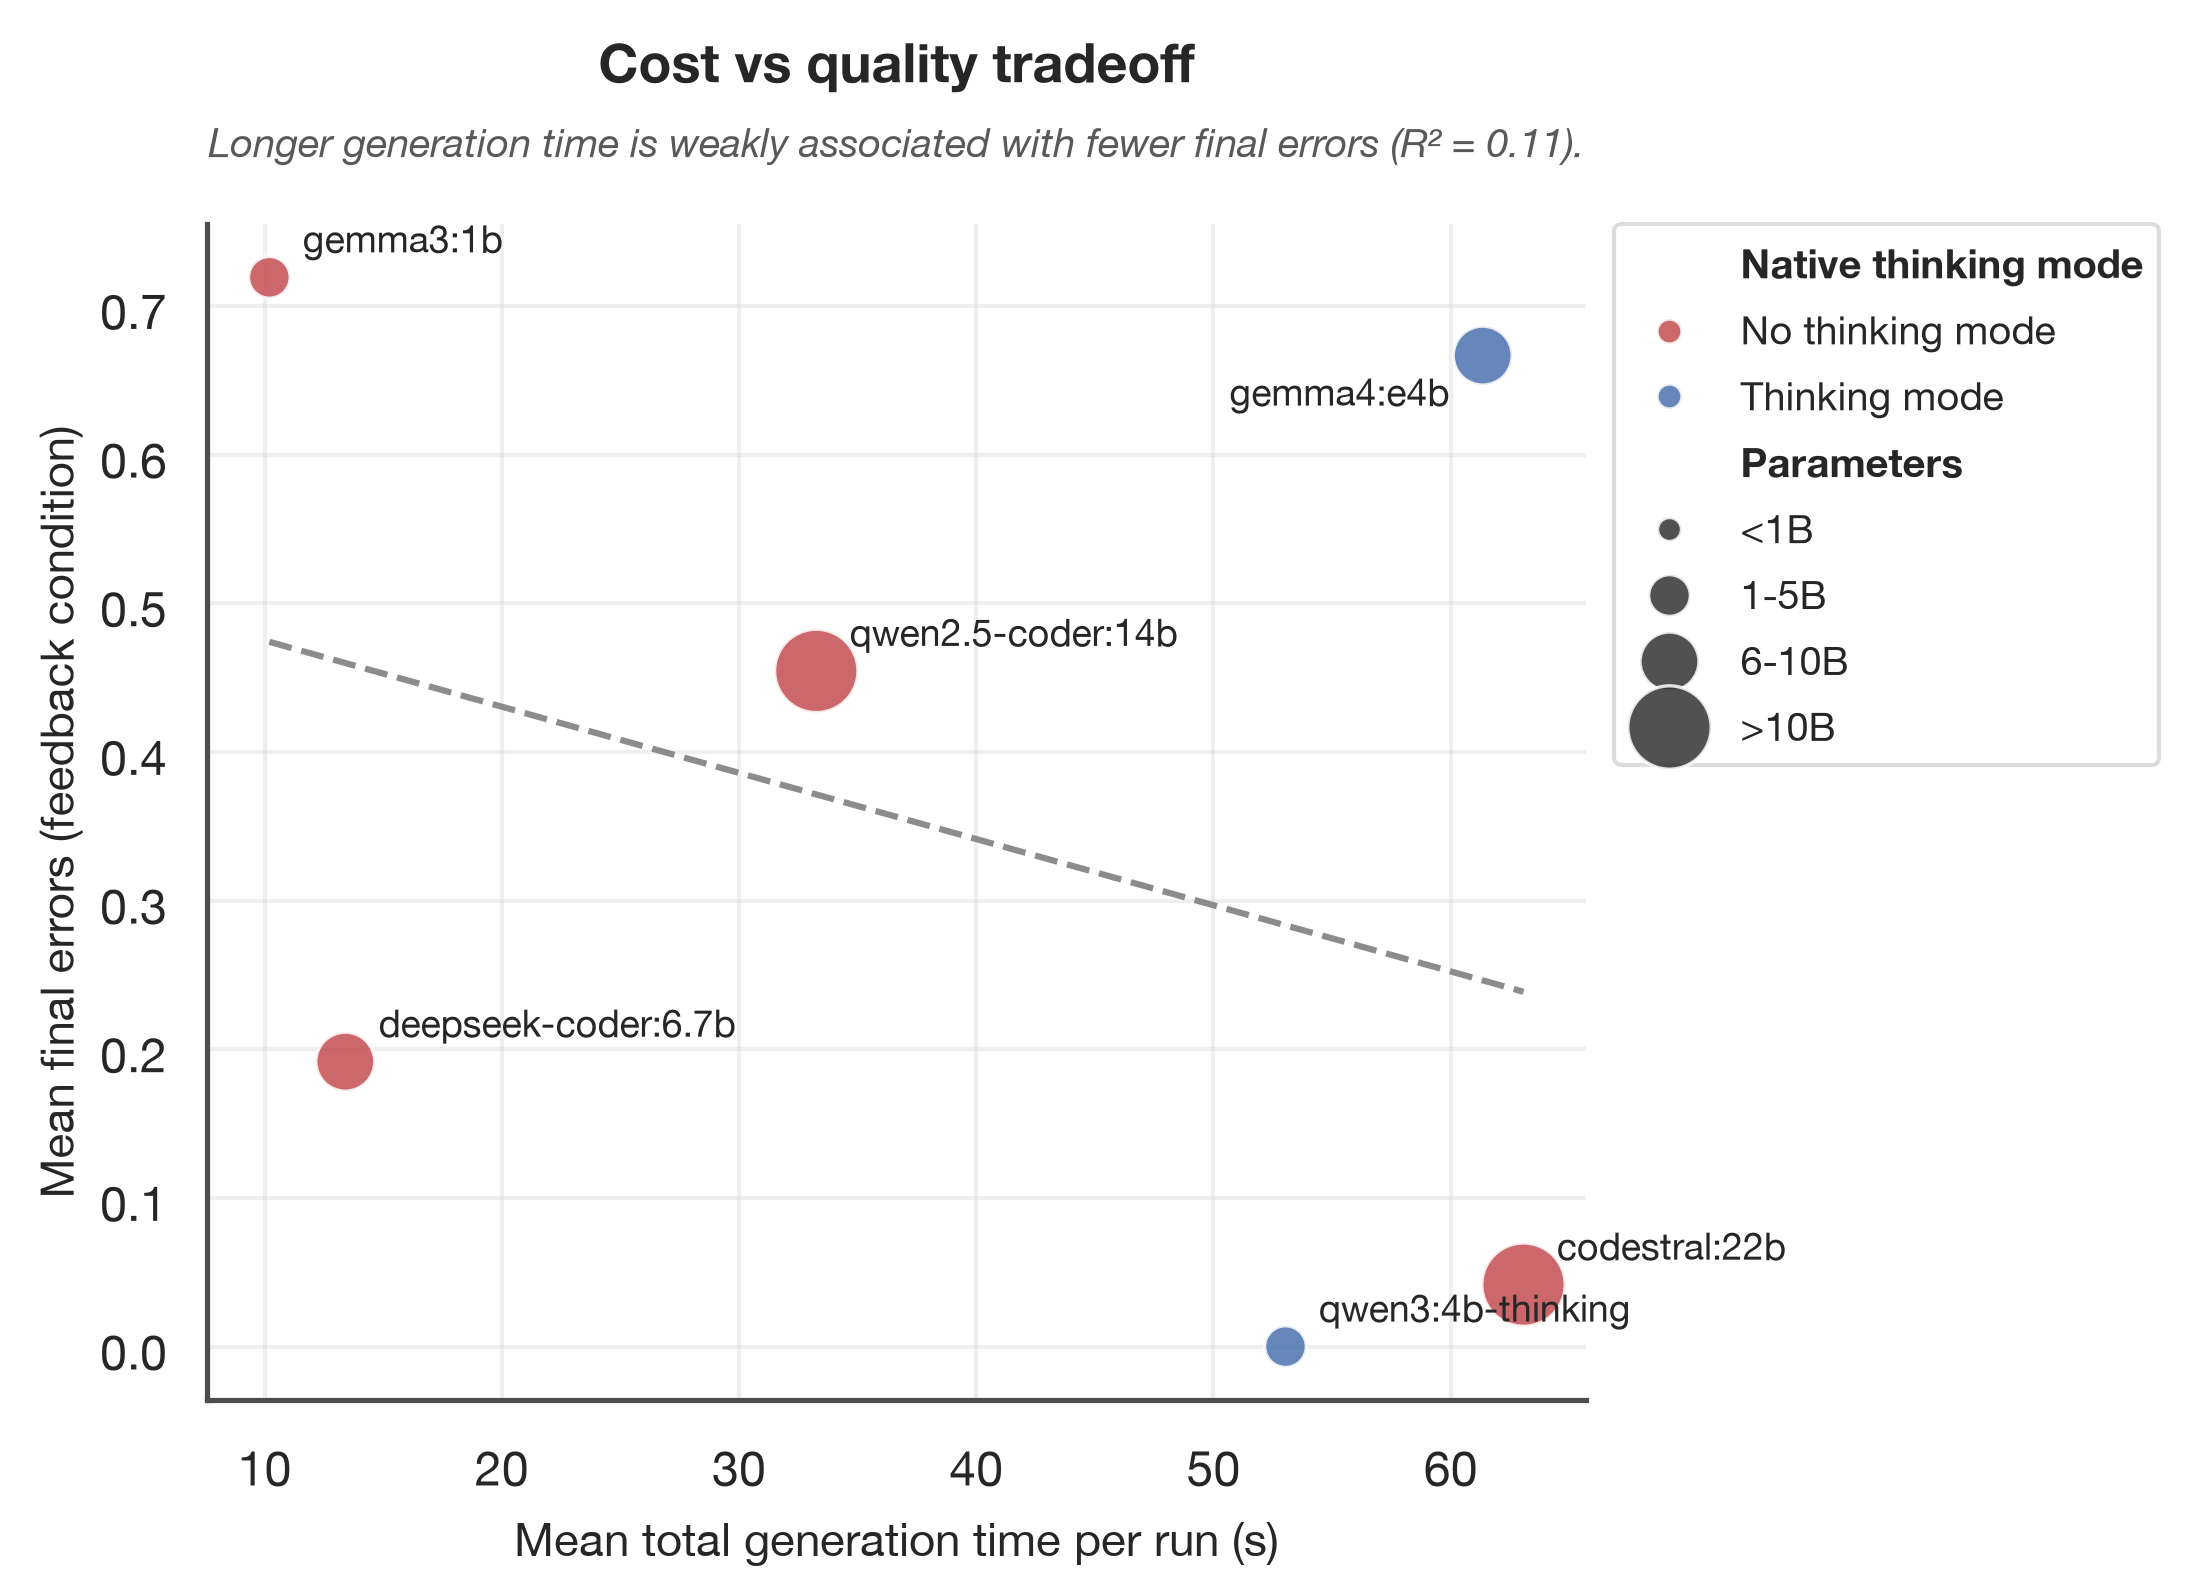
\includegraphics[width=0.85\linewidth]{images/cost_quality_errors.png}
	\caption{Mean total generation time per run vs mean final error count (feedback condition), one point per model. Colour encodes native thinking mode, point size encodes parameter-count bin.}
	\label{fig:cost-quality}
\end{figure}
\begin{figure}[H]
	\centering
	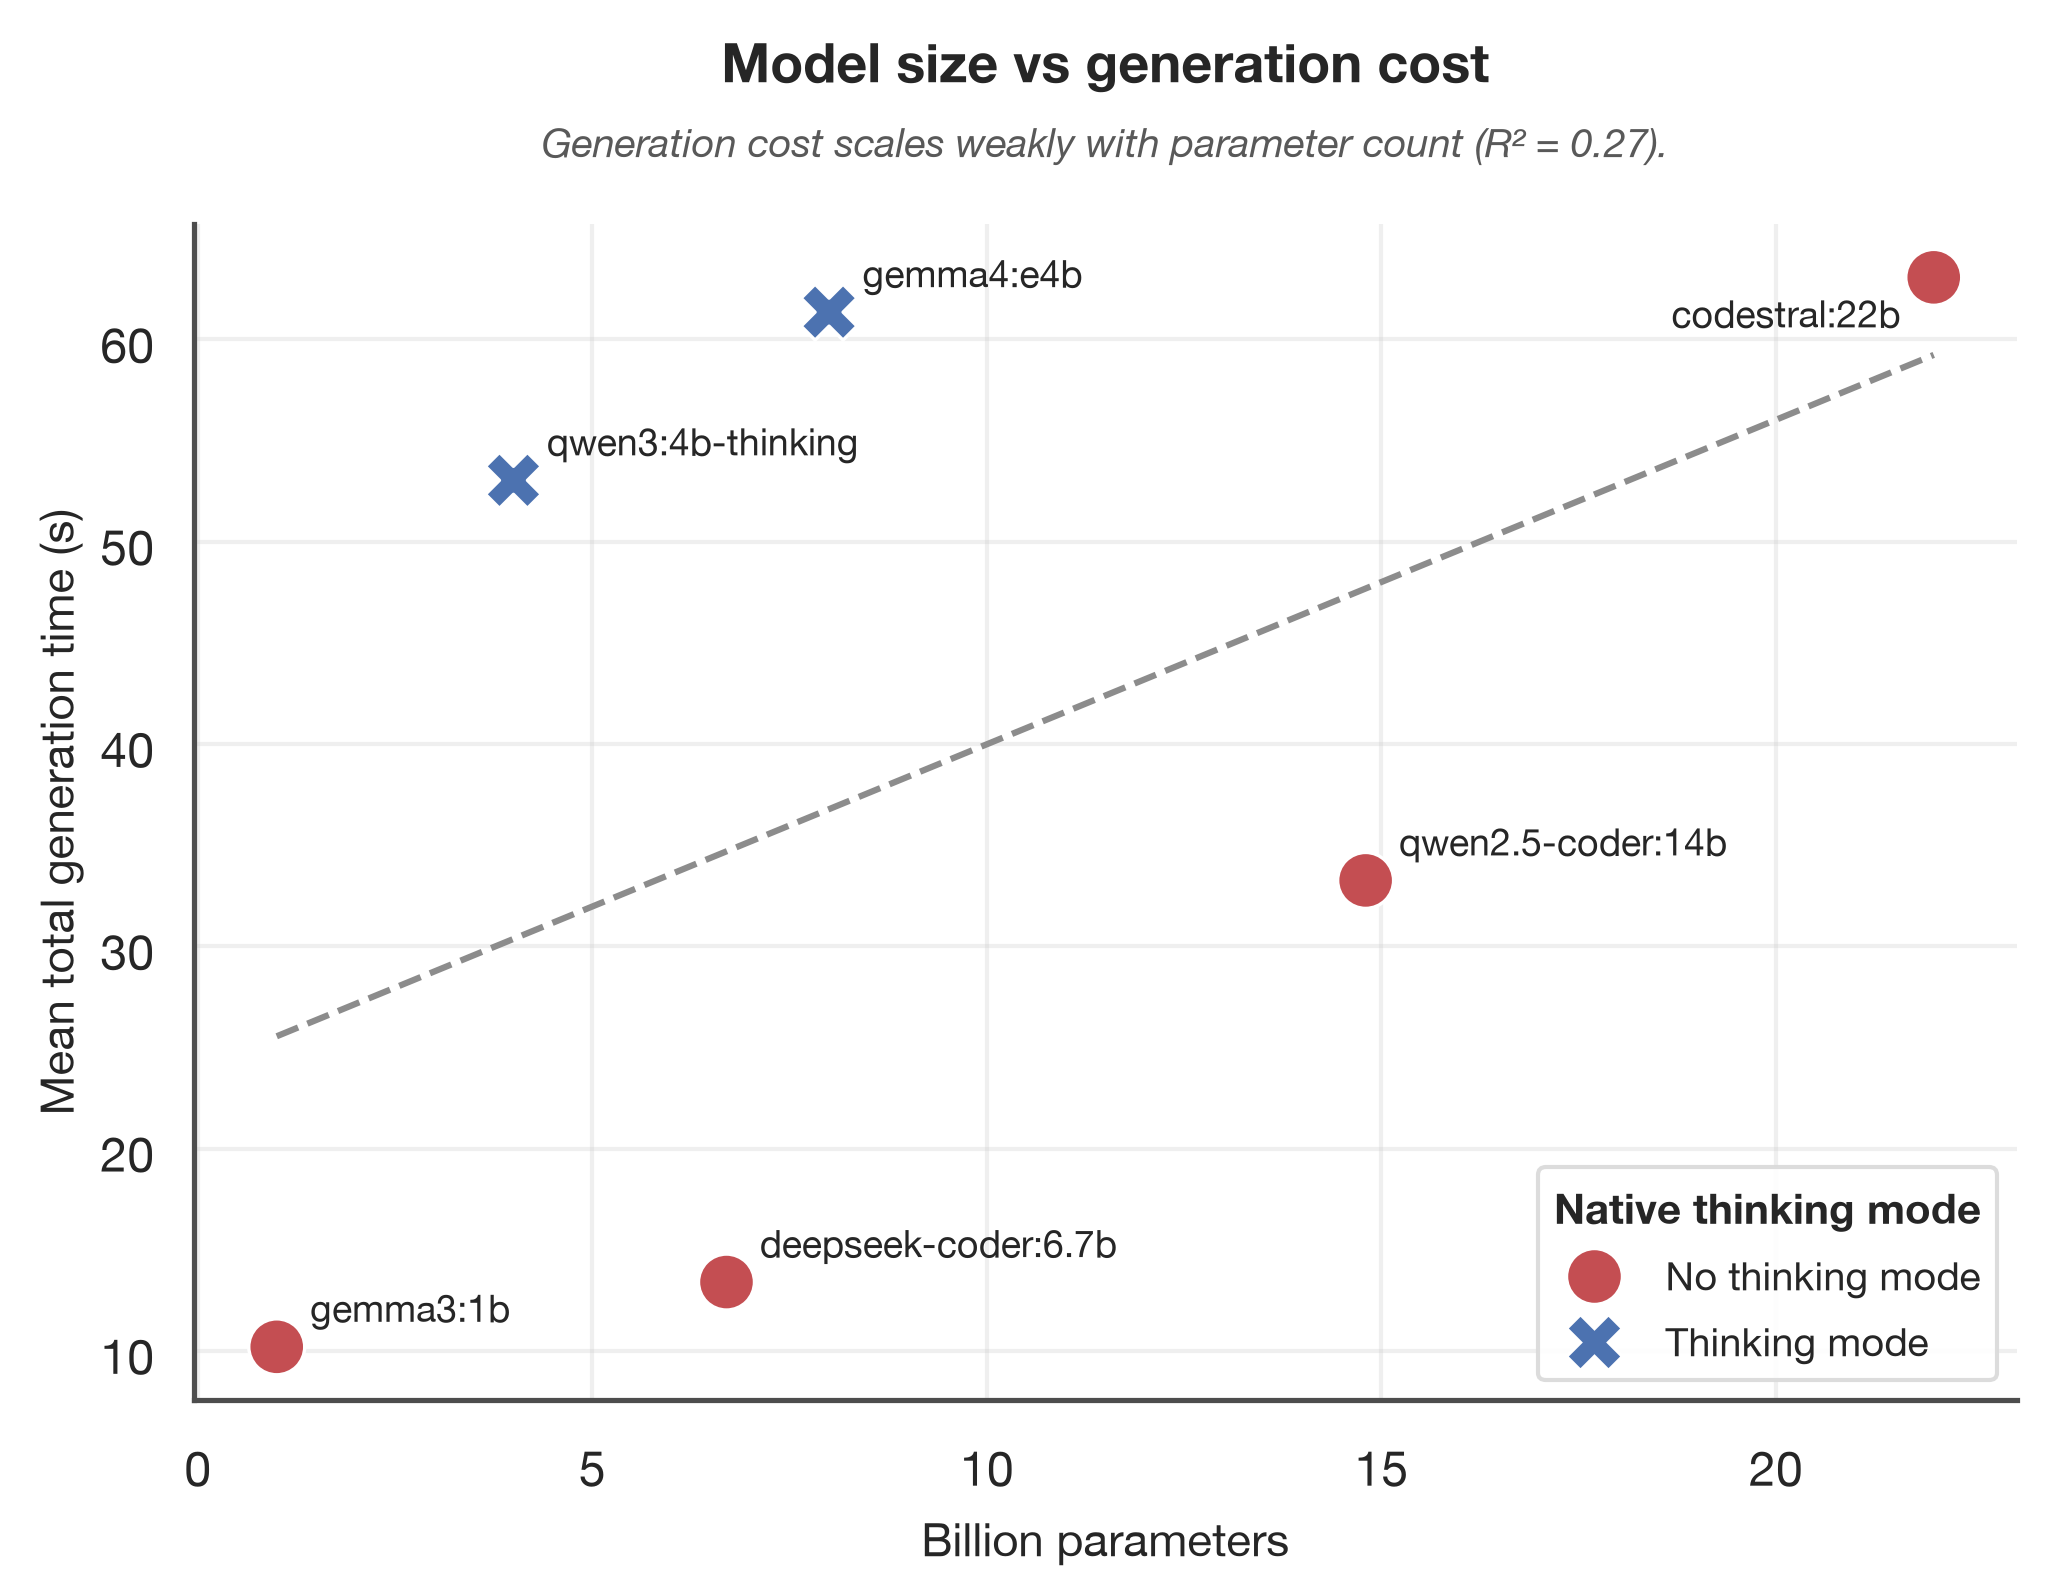
\includegraphics[width=0.7\linewidth]{images/model_size_vs_cost_errors.png}
	\caption{Parameter count vs mean total generation time per run, coloured by native thinking mode.}
	\label{fig:model-size-vs-cost}
\end{figure}

% = PARAGRAPH 3 = Reasoning vs. non-reasoning as the decisive variable

Give this finding its own paragraph because it is the most interesting and surprising result of RQ2. Explicitly compare a smaller reasoning model against codestral:22b. If a reasoning model with fewer parameters achieves better error reduction in fewer iterations at lower latency, that is a concrete, reportable conclusion that directly challenges the assumption that more parameters equal better output.

\begin{figure}[H]
	\centering
	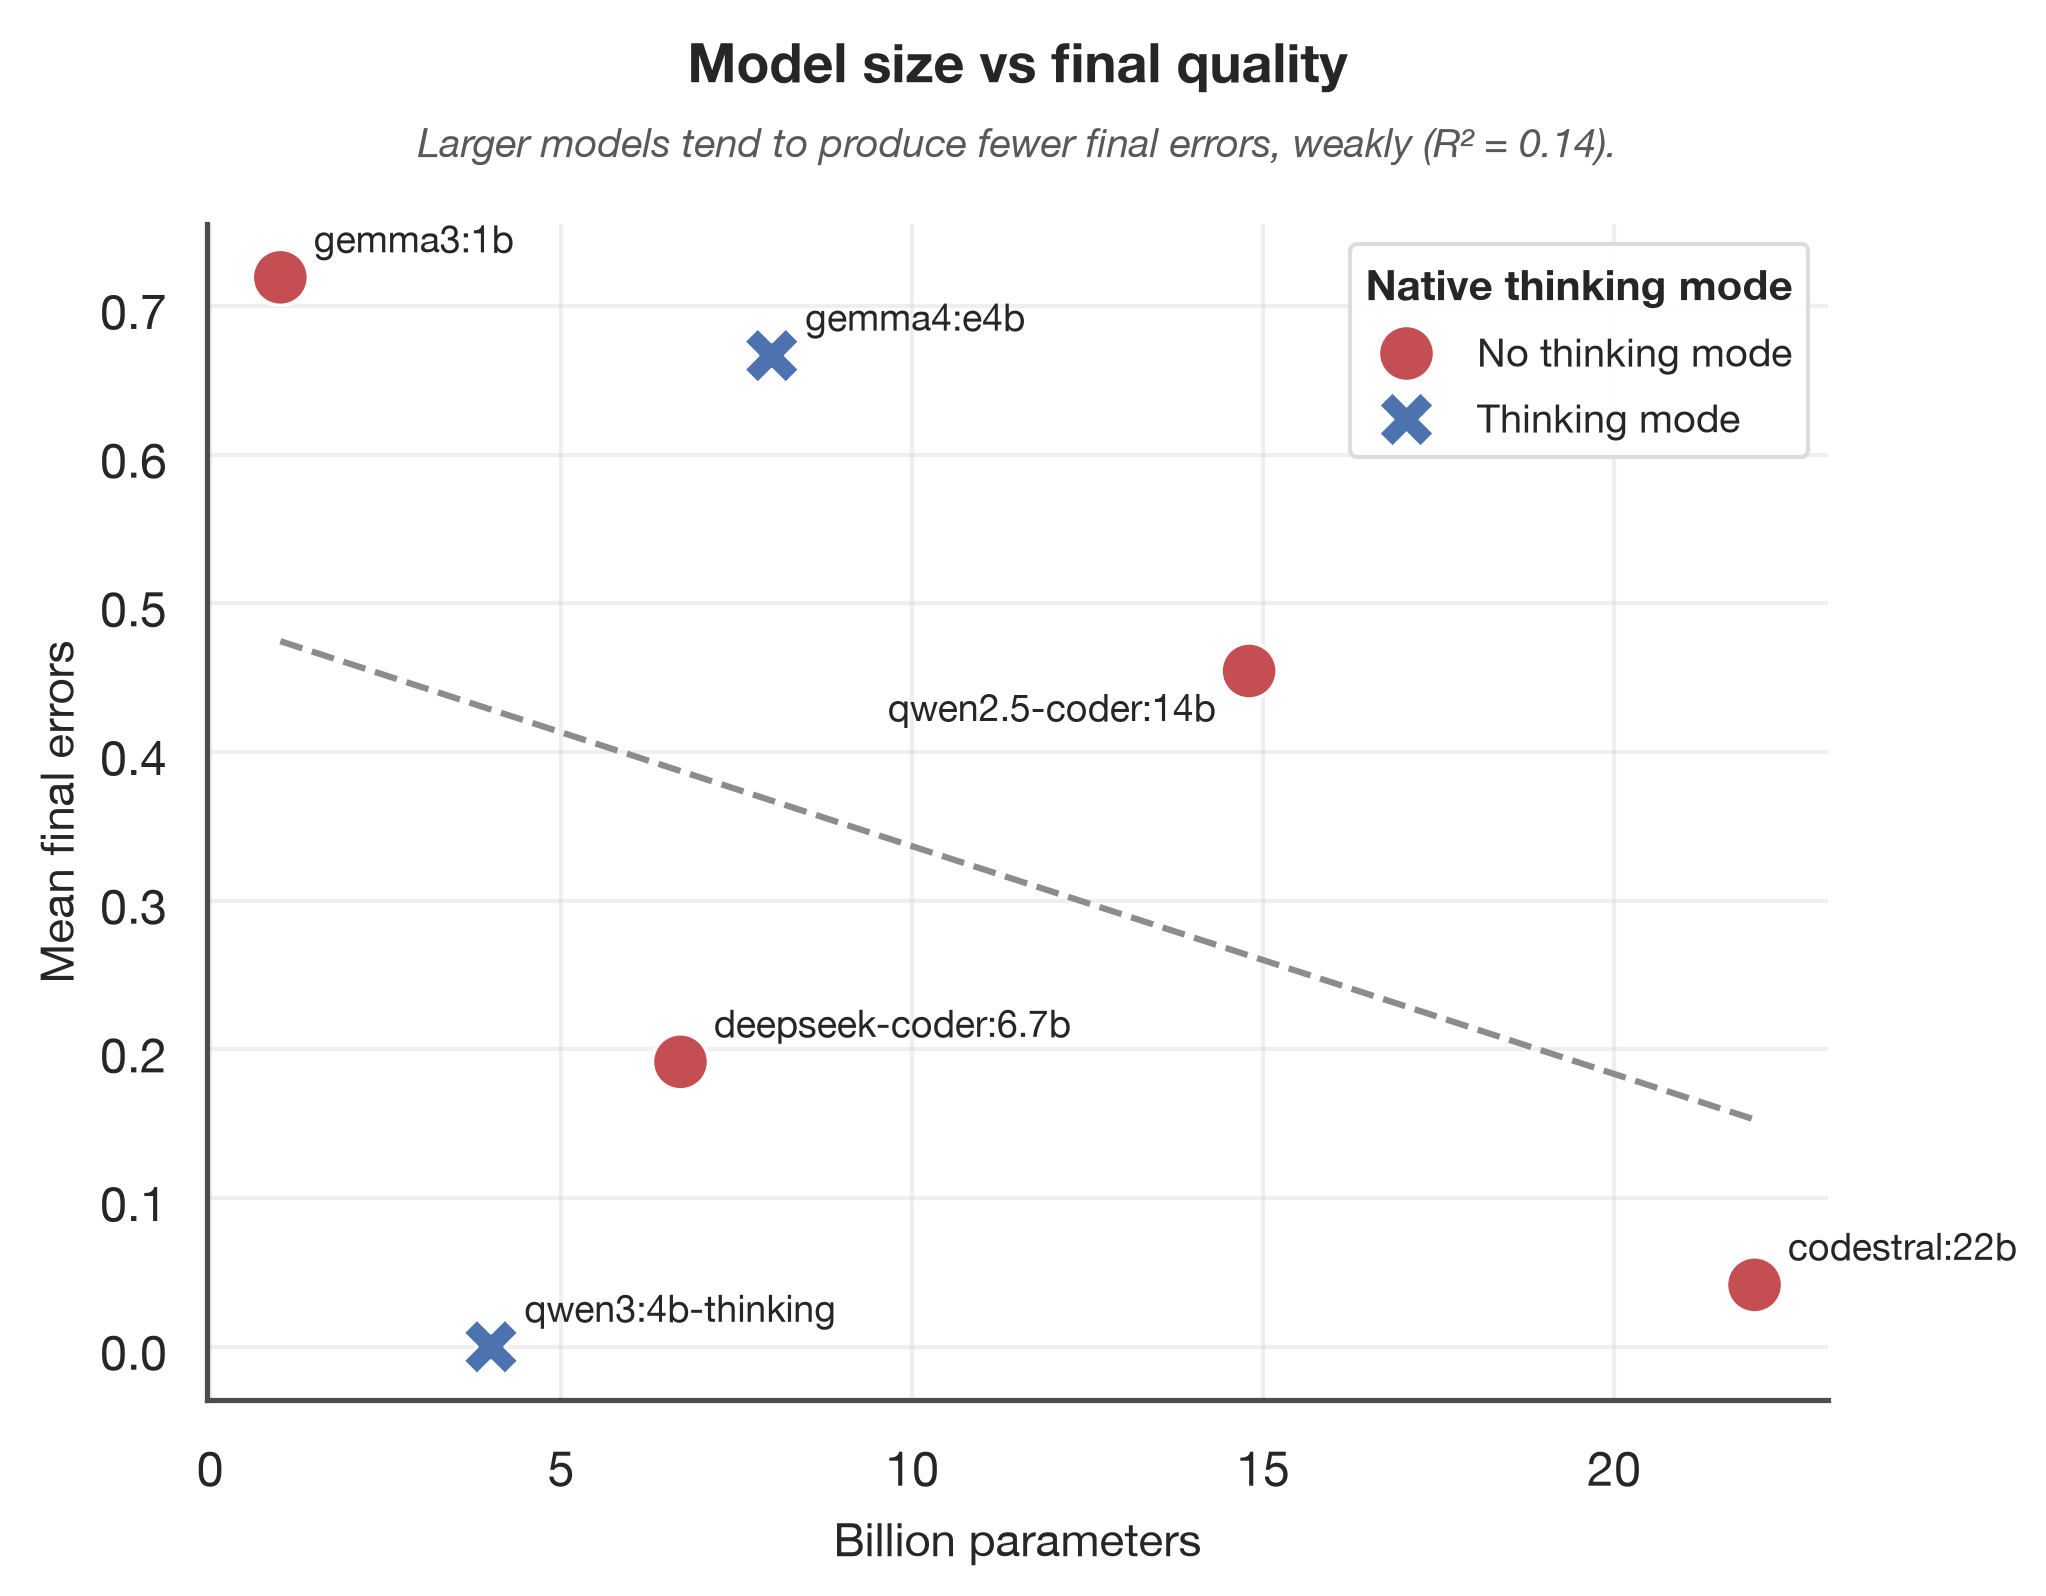
\includegraphics[width=0.7\linewidth]{images/model_size_vs_quality_errors.png}
	\caption{Parameter count vs mean final error count (feedback condition), coloured by native thinking mode. qwen3:4b-thinking (4B, reasoning) reaches a lower mean final error count than codestral:22b (22B, non-reasoning) at roughly a fifth of the parameters.}
	\label{fig:model-size-vs-quality}
\end{figure}

% = PARAGRAPH 4 = Cost of the feedback loop vs. the blind condition

Does the \verb|feedback| condition cost more than \verb|blind| in token terms? It should, since it passes longer prompts (original code + error list). Is the extra cost justified by the quality gain? Frame this as a cost-benefit ratio: additional tokens spent per additional error resolved.

% Answer worth checking before writing this paragraph: per analysis.stats.token_cost_comparison, feedback is actually CHEAPER than blind in total tokens per run for 5 of 7 models (and pooled across all models) -- not more expensive as assumed above. This is because blind converges more slowly (more reprompt iterations needed on average, each carrying its own token cost), so even though each individual feedback iteration's prompt is longer (original code + specific error list), feedback needs fewer of them. Confirm this holds before writing the "it should cost more" framing as-is.
% Cost-benefit table: see tables.tex, Table~\ref{tab:rq2-token-cost} (tab:rq2-token-cost).



\subsection{Iteration Count Analysis}

% When does the loop converge? Is there a diminishing return after N iterations? This is where you answer the "optimal number of iterations" question.

% \textbf{Change}: No major structural change, but the analysis now comes from \verb|stats.py|'s iteration-cutoff analysis, which is worth naming explicitly as the source of the convergence findings.

% = PARAGRAPH 1 = Convergence behaviour

Using the output of \verb|stats.py|'s iteration-cutoff analysis, describe when models typically converge. Do most runs resolve within 1-2 iterations, or does error reduction continue meaningfully up to the maximum? Present a distribution (histogram or line chart) of iterations-to-convergence across all (model, prompt) pairs in the \verb|feedback| condition.

\begin{figure}[H]
	\centering
	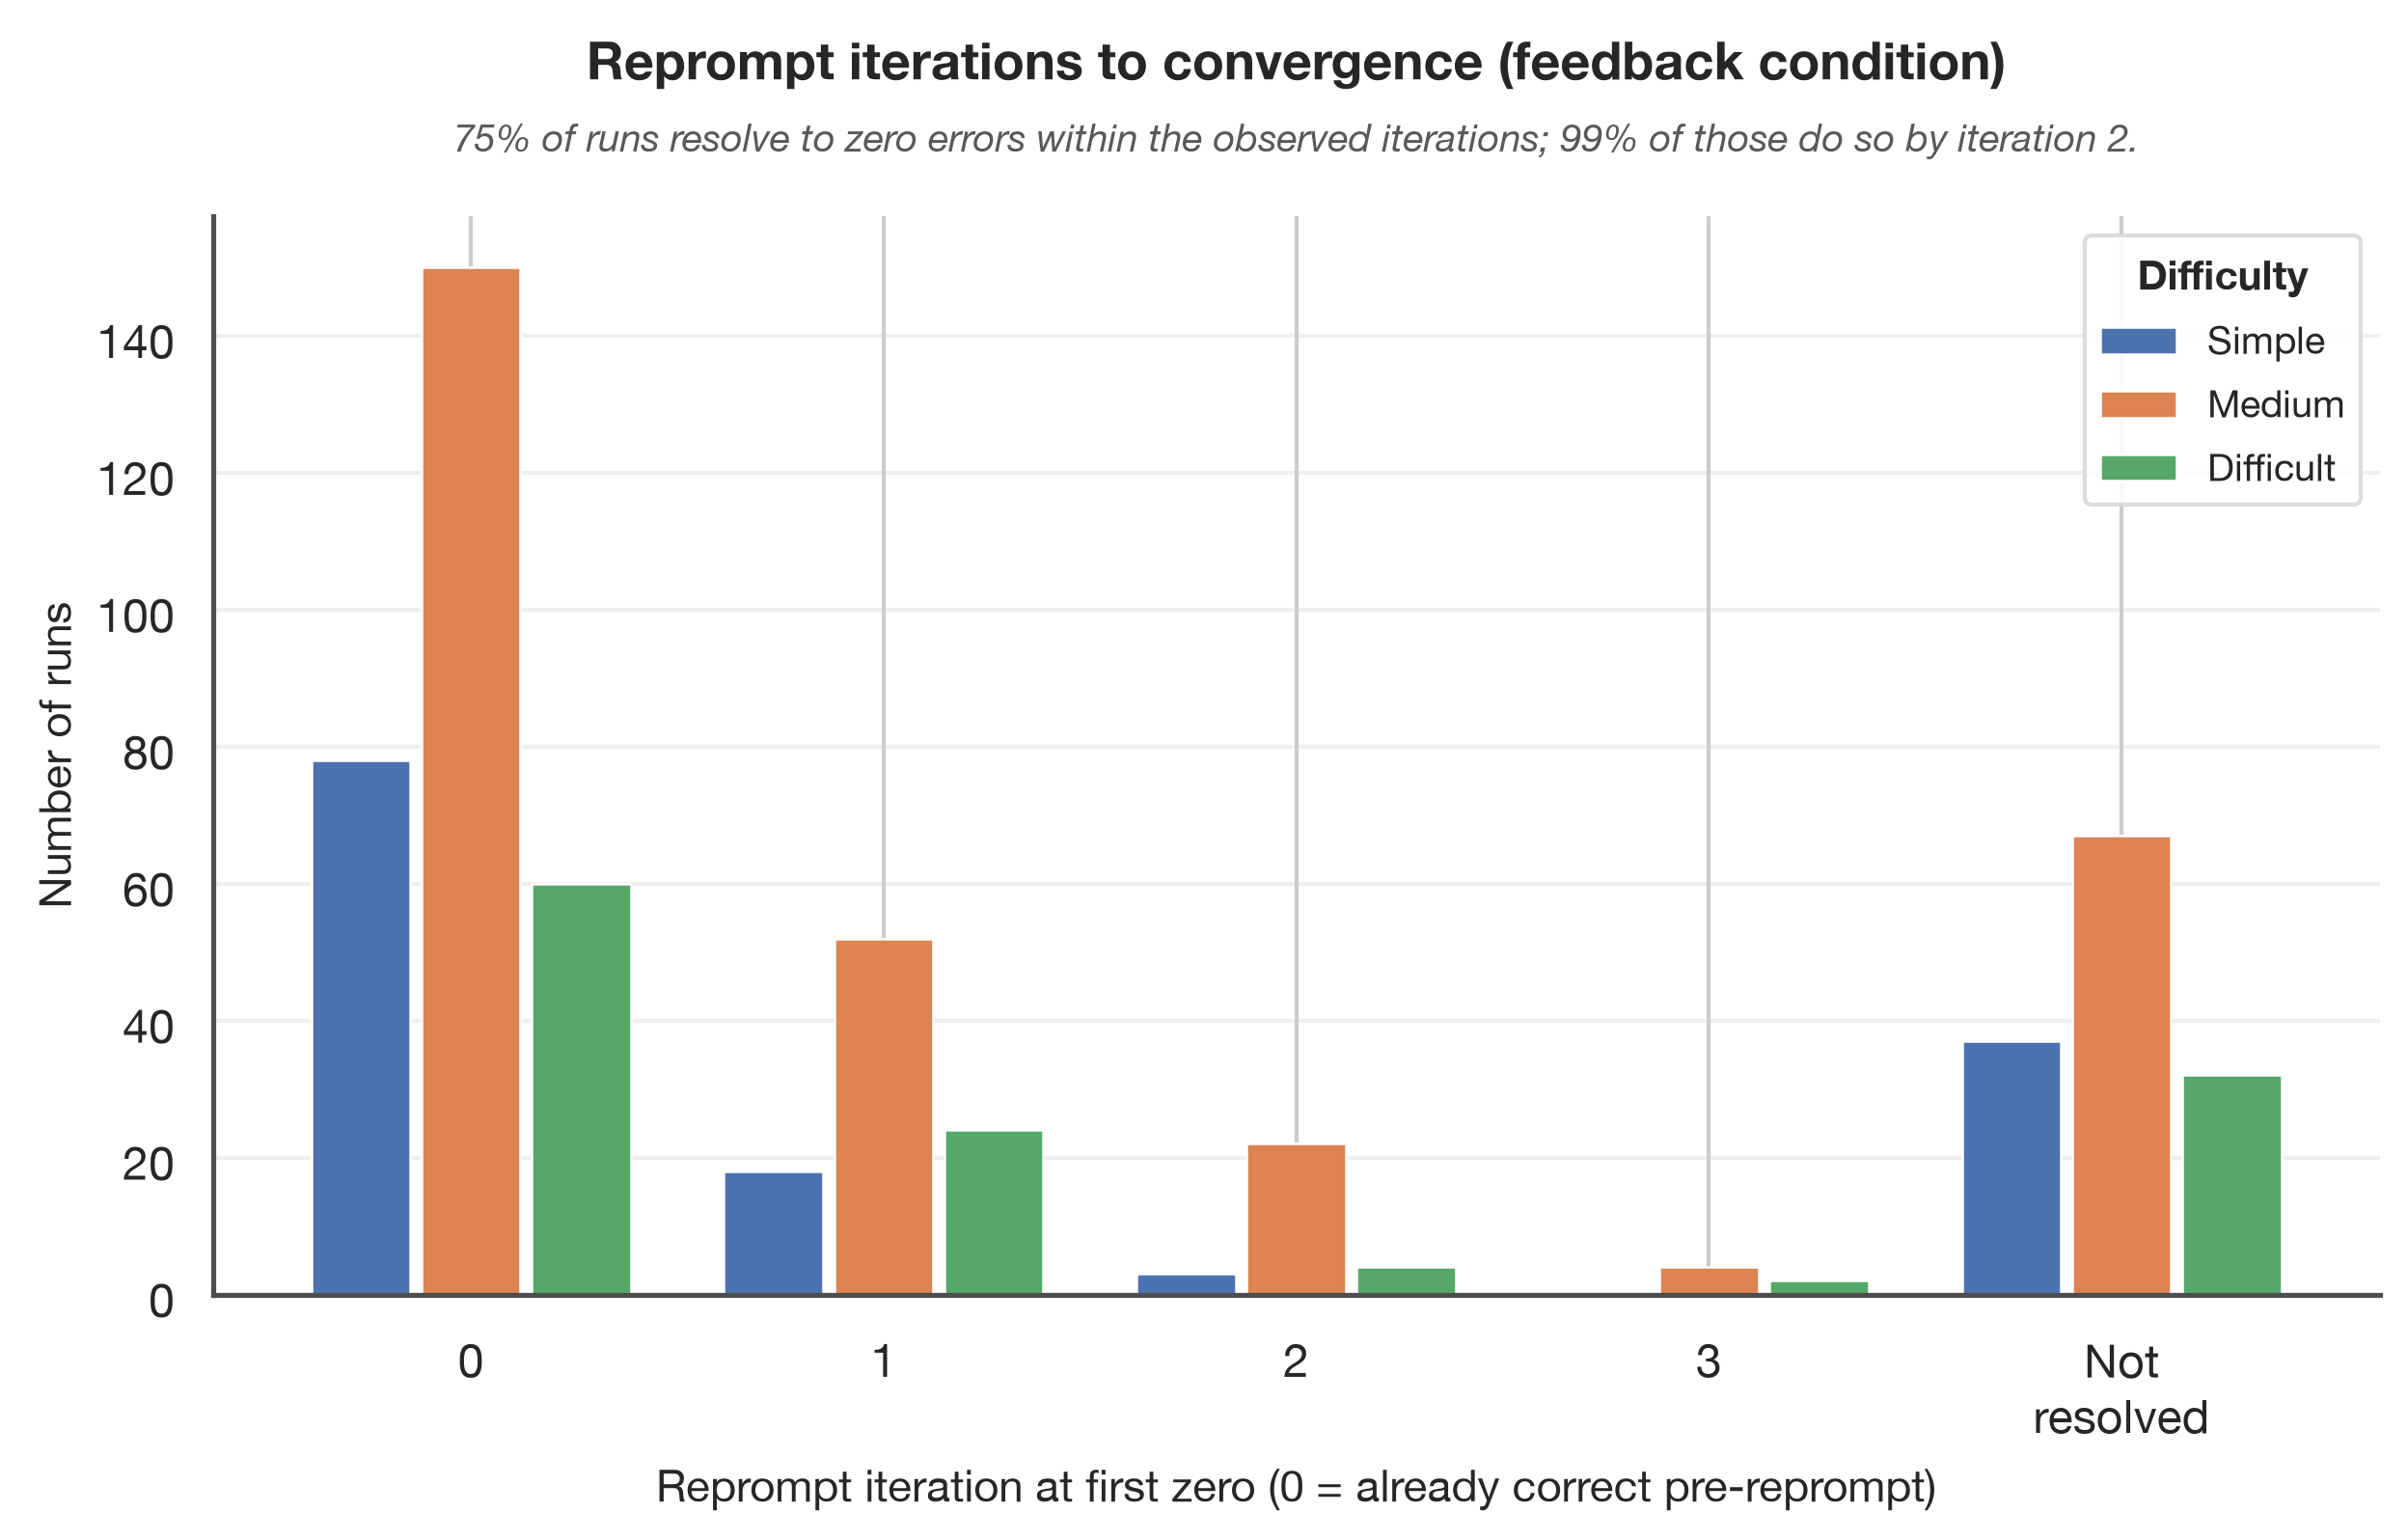
\includegraphics[width=\linewidth]{images/iteration_convergence_errors.png}
	\caption{Distribution of the reprompt iteration at which each (model, prompt, trial) run first reaches zero errors, feedback condition, split by prompt difficulty tier. ``Not resolved'' = still nonzero at the last observed iteration.}
	\label{fig:iteration-convergence}
\end{figure}

% = PARAGRAPH 2 = Dimishing returns and the optimal cut-off

Identify where the marginal gain per additional iteration drops below a meaningful threshold. If, for example, 80\% of resolvable errors are fixed by iteration 2 and iterations 3-5 contribute minimally, that is your practical recommendation for the maximum iteration count. State this as a concrete finding rather than a vague observation. Note whether this threshold differs by model or difficulty tier.

% Cutoff-by-difficulty table: see tables.tex, Table~\ref{tab:iteration-cutoff-difficulty} (tab:iteration-cutoff-difficulty). Per-model cutoff table is the same function with group_by="model" (not pre-generated into tables.tex since it has one row per model per cutoff -- regenerate via analysis.stats.iteration_cutoff_analysis if you want it tabulated too).

\section{Discussion (2 \textendash{} 3 pages)}
\label{sec:discussion}

\section{Conclusion (0.5 \textendash{} 1 page)}
\label{sec:conclusion}



% \bibliographystyle{plainnat}
\bibliography{references}

% (optional) APPENDIX
\appendix
\section*{Appendix}
\label{sec:appendix}


\subsection*{Full prompt dataset}
\subsection*{Extended results tables}
\subsection*{Flowchart (if not in main body)}
\subsection*{Human evaluation rubric (if used)}
\subsection*{Project timeline} % dont think this is necessary


\begin{itemize}
	\item Full prompt dataset
	\item Extended results tables
	\item Flowchart (if not in main body)
	\item Human evaluation rubric (if used)
	\item Project timeline — your supervisor asked for this; an appendix is a natural place for if it doesn't fit in the main body
\end{itemize}



\end{document}
